\section{Detection Using White Spaces and Recognition Using CNN}

\setcounter{figure}{0}
\renewcommand{\thefigure}{6.\arabic{figure}}

\subsection{Detection}
For the CNN methods the detection process is very important as it provides the CNN model with an image for every character in the page to be translated, this is done by the manipulation of pixels color information providing a reliable dividing process. 
\subsubsection{Turning the image into zeros and ones}
After the preprocessing stage the output page consists of black and white colors only, the value of each pixel is extracted from the page forming a 2D array the same size of the page to be translated, each cell contains either value 1 if the corresponding pixel is black or 0 if the corresponding pixel is white.
\begin{figure}[!ht]
    \centering
    \subfloat[Input demo image]{\includegraphics[width=0.5\linewidth]{6.1.1.png}}\hfill
    \subfloat[2D array of the input image]{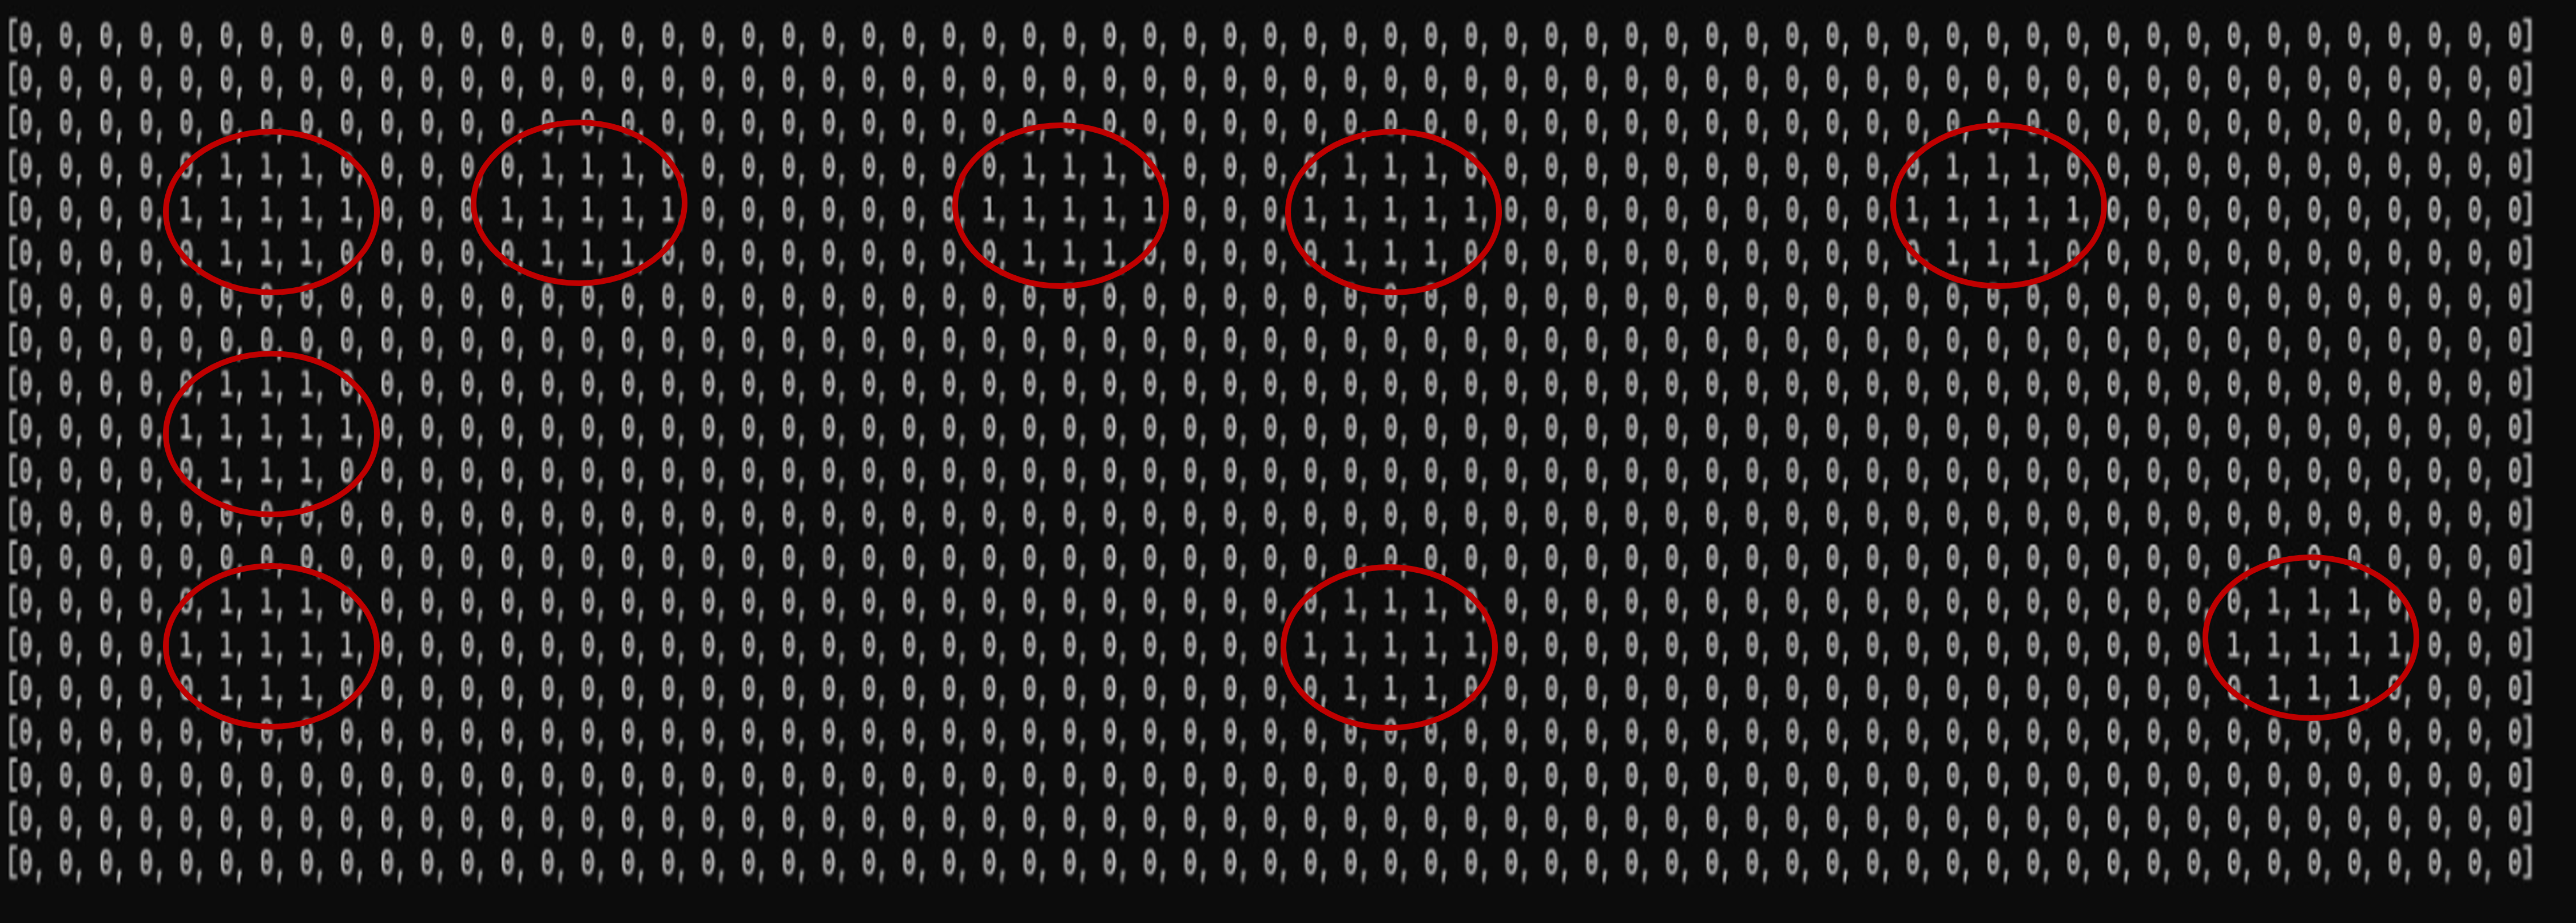
\includegraphics[width=1\linewidth]{6.1.13.png}}\\
    \caption{Making a 2D array of zeros and ones from the input image}
    \label{fig:Making a 2D array of zeros and ones from the input image}
\end{figure}

\subsubsection{Determining the existence of black pixels}
The values of cells for each row are summed up and for each column. That gives us the information about which row and which column may have a black pixel.
\subsubsection{Deciding the candidate coordinates}
A suitable constant threshold is selected for the configuration we are working with. The threshold is used for the elimination of rows and columns that contains noise or not enough numbers of black pixels. This gives us the coordinates of the rows and columns which contains a convenient  number of black pixels, and we assign a value for that coordinate.

\clearpage
\begin{figure}[!ht]
\centering
\includegraphics[width=1\linewidth]{6.1.3.png}
\caption{Rows coordinates array after assigning values}
\label{fig:rows coordinates array after assigning values}
\end{figure} 
Using the variance of that value we could determine the coordinate where the whole black dot started and the coordinate where it ended, we utilize these coordinates by taking a step left or right in case of column or a step up and down in case of rows by specific amount determined by the dynamic of coordinates variance to determine every row and column that is a start of a whole braille dot or the end of it.
\begin{figure}[!ht]
\centering
\includegraphics[width=0.7\linewidth]{6.1.4.png}
\caption{Selecting columns and rows coordinate surrounding braille dots}
\label{fig:selecting columns and rows coordinate surrounding braille dots}
\end{figure} 
\begin{figure}[!ht]
    \centering
    \subfloat[selected columns surrounding braille dots (purple is shared coordinate)]{\includegraphics[width=0.4\linewidth]{6.1.5.png}}\hfill
    \subfloat[selected rows surrounding braille dots]{\includegraphics[width=0.4\linewidth]{6.1.6.png}}\\
    \caption{Selected rows and columns surrounding braille dots}
    \label{fig:Selected rows and columns surrounding braille dots}
\end{figure}

\subsubsection{Extracting symbols coordinates}
As each braille symbol contain three rows and two columns, we select the coordinates that contain the whole braille symbol not just a dot by jumping 4 coordinates in case of rows and 2 coordinates in case of columns.
\begin{figure}[!ht]
    \centering
    \subfloat[symbols coordinates array]{\includegraphics[width=0.3\linewidth]{6.1.7.png}}\hfill
    \subfloat[selected coordinates surrounding braille symbols]{\includegraphics[width=0.6\linewidth]{6.1.8.png}}\\
    \caption{Extracting symbols coordinates}
    \label{fig:Extracting symbols coordinates}
\end{figure}

\newpage
\subsubsection{Dividing the page into symbol images}
By iterating the coordinates we extracted from the previous step we iterate each symbol by the four coordinates that holds it, then the images are cropped and passed to the next stage of recognition in order. The dividing was not efficient in case of rotated pages as the process of aligning changed the size of the dots which the threshold is calibrated on, resulting incorrect divisions for some lines, which lead to use of straightened pages only with the CNN approach.

\begin{figure}[!ht]
\centering
\includegraphics[width=1\linewidth]{6.1.9.png}
\caption{samples of divided braille symbols from the first rows of a page}
\label{fig:samples of divided braille symbols from the first rows of a page}
\end{figure} 

\subsubsection{Problems and Challenges }
\paragraph{Eliminating unnecessary Extra points }\par
there are some occasions where the user differentiate from the standard form of the Braille symbol and print the symbol with 4 rows instead of 3, which results in ruining the whole order of the coordinates as we work with only the standard form of 6 Braille dots. This was solved by eliminating the Extra points from the array either by the threshold and considering it as noise or by calculating the distance between it and the previous row, as the first row after three rows should have a bigger distance than the fourth row.
\begin{figure}[!ht]
\centering
\includegraphics[width=0.35\linewidth]{6.1.10.png}
\caption{the variation of vertical distances between fault and normal dots}
\label{fig:the variation of vertical distances between fault and normal dots}
\end{figure} 

\paragraph{Page number fading with threshold}\par
this problem occur as the symbol of the number is always in a whole number of rows alone with no other symbols, so threshold that eliminate noise remove it. To solve this we implemented dynamic threshold, it starts small at the top of the page to pass the number symbol then it returns to the constant threshold which is suitable for the rest of the page.


\begin{figure}[!ht]
\centering
\includegraphics[width=0.8\linewidth]{6.1.11.png}
\caption{the page number symbol in a whole line }
\label{fig:the variation of vertical distances between fault and normal dots}
\end{figure} 








\subsection{Datasets}
In our project, we used two different datasets: one was downloaded from the Kaggle website [15], and the other was created by us. This section will discuss the domains of these datasets.
\subsubsection{Kaggle Dataset}
\begin{enumerate}
    \item \textbf{Description:} 
    This dataset was sourced from the Kaggle website and has been utilized in numerous projects. It comprises images of 26 characters, each represented by 60 images of size 28x28 pixels, with various augmentations (including different shifts, rotations, and brightness values). The labels for the images are the letters from A to Z.
    \item \textbf{Samples:}
    Figures \ref{fig:data1}(a), \ref{fig:data1}(b), \ref{fig:data1}(c), and \ref{fig:data1}(d) show the symbol representing the letter A with different augmentations in this dataset.

\begin{figure}[!ht]
\centering
\subfloat[Brightness changed.]{\includegraphics[width=0.45\linewidth]{brightness.jpg}}\hfill
\subfloat[Shifted.]{\includegraphics[width=0.45\linewidth]{shift.jpg}}\\
\subfloat[Rotated 45 degrees]{\includegraphics[width=0.45\linewidth]{rot1.jpg}}\hfill
\subfloat[Rotated -90 degrees]{\includegraphics[width=0.45\linewidth]{rot2.jpg}}
\caption{Letter A in Braille}
\label{fig:data1}
\end{figure}

    \item \textbf{Problems:}
    \begin{enumerate}
        \item The dataset does not cover all possible combinations of Braille characters.
        \item Some images are rotated at large angles or flipped, causing symbols to resemble others, which decreases the model's accuracy.
        \item The most significant issue is that symbols detected from an entire Braille-written page appear very different from the images in the dataset, preventing the model from recognizing them.
    \end{enumerate}

\end{enumerate}

To overcome these issues, we decided to create our own dataset.

\subsubsection{Custom Dataset}
To obtain a dataset that meets our needs, we created our own dataset using the detection of symbols with white spaces as discussed in the previous section.

\begin{enumerate}
    \item \textbf{Description:} 

    To generate this dataset we used four Braille one-sided pages and we conducted two trials. In the first trial, we used detection in image processing, as discussed in Chapter Five, which produced labeled images for each character. However, we did not use this dataset because the properties of the generated images did not match those of the images that would be used with the model.
    
    In the second trial, we used detection using white spaces, as discussed in the previous section. This method generated unlabeled images, which we then labeled manually. The properties of these images closely matched what we needed. Therefore, the dataset was generated from the second trial.

    
    Initially, the dataset was unbalanced; some symbols had many images while others had only one. To address this imbalance, we applied data augmentation techniques. We augmented the images by shifting, changing brightness, and rotating them at small angles not exceeding 10 degrees to avoid altering the symbol’s shape, among other methods. After augmentation, the dataset comprised 6519 images, with each symbol represented by about 100 images of size 224x224 pixels.The images were labeled as zeros and ones, corresponding to the arrangement of dots as illustrated in the introduction in chapter 1.
        
    \item \textbf{Samples:}
Figures \ref{fig:data}(a), \ref{fig:data}(b), \ref{fig:data}(c), and \ref{fig:data}(d) are samples from our dataset. Figure \ref{fig:data}(a) represents the space, while figures \ref{fig:data}(c) and \ref{fig:data}(d) depict the same symbol; however, noise has been added to the second image.

\begin{figure}[!ht]
\centering
\subfloat['000000']{\includegraphics[width=0.45\linewidth]{2_000000_1.png}}\hfill
\subfloat['010011']{\includegraphics[width=0.45\linewidth]{0_010011_1.png}}\\
\subfloat['001111']{\includegraphics[width=0.45\linewidth]{4_001111.png}}\hfill
\subfloat['001111' with noise]{\includegraphics[width=0.45\linewidth]{4_001111_1.png}}
\caption{Samples from Custom dataset}
\label{fig:data}
\end{figure}
\end{enumerate}

\subsection{Convolutional Neural Network Models}

\begin{figure}
\centering
\includegraphics[width=\linewidth]{cnn.PNG}
\caption{CNN architecture}
\label{fig:cnn}
\end{figure}

A Convolutional Neural Network (CNN or ConvNet) is a class of neural networks that specializes in processing data with a grid-like topology, such as images. A digital image is a binary representation of visual data, consisting of pixels arranged in a grid. Each pixel contains values that indicate its brightness and color. A typical CNN comprises three types of layers: convolutional layers, pooling layers, and fully connected layers as shown in Figure \ref{fig:cnn}

\begin{enumerate}
    \item \textbf{Convolution Layer:} The convolution layer is the core building block of the CNN. It carries the main portion of the network’s computational load.
    \item \textbf{Pooling Layer:} The pooling layer replaces the output of the network at certain locations by deriving a summary statistic of the nearby outputs. This helps in reducing the spatial size of the representation, which decreases the required amount of computation and weights. The pooling operation is processed on every slice of the representation individually.
    \item \textbf{Fully Connected Layer:} Neurons in this layer have full connectivity with all neurons in the preceding and succeeding layers, similar to what is observed in regular Fully Connected Neural Networks (FCNN). Consequently, it can be computed as usual through matrix multiplication followed by the addition of a bias term. The Fully Connected (FC) layer helps map the representation between the input and the output.
    \item \textbf{Non-Linearity Layers:} Since convolution is a linear operation and images are far from linear, non-linearity layers are often placed directly after the convolution layer to introduce non-linearity to the activation map.
\end{enumerate}

This is a brief explanation of Convolutional Neural Networks (CNNs) in general. In the following sections, we will focus on the specific models we used: one model that we built ourselves, and another that utilized a pretrained model called DenseNet201.

\subsubsection{Custom Model}
In this section, we describe the architecture and design of the model built by ourselves. 
\begin{enumerate}
    \item \textbf{Model architecture:} Our model, constructed using the Keras Sequential API, includes the following layers, as illustrated in the block diagram in Figure \ref{fig:custom model}:

\begin{figure}[!ht]
\centering
\subfloat[The complete model]{\includegraphics[width=\linewidth]{model.jpg}}\hfill
\subfloat[First Convolutional Block]{\includegraphics[width=0.45\linewidth]{first block.PNG}}\\
\subfloat[Second,third \& forth Convolutional Blocks]{\includegraphics[width=0.45\linewidth]{second.PNG}}\hfill
\subfloat[Fully Connected Layers]{\includegraphics[width=\linewidth]{fullyconnected.PNG}}
\caption{Custom model block diagram}
\label{fig:custom model}
\end{figure}


    \begin{enumerate}
        \item Input Layer: The input layer is configured to accept grayscale images with a shape of 224x224 pixels and a single color channel.
        
        \item First Convolutional Block:

        \textbf{Conv2D Layer:} 64 filters, 5x5 kernel size, 'same' padding, ReLU activation, and L2 regularization to prevent overfitting.
        
        \textbf{BatchNormalization:} Normalizes the outputs of the convolutional layer to speed up training and improve stability.
        
        \item Second Convolutional Block:

        \textbf{Conv2D Layer:} 64 filters, 3x3 kernel size, 'same' padding, ReLU activation, and L2 regularization.
        
        \textbf{BatchNormalization:} Normalizes the outputs of the convolutional layer.
        
        \textbf{MaxPooling2D:} Reduces the spatial dimensions of the feature maps.
        
        \item Third Convolutional Block:

        \textbf{Conv2D Layer:} 64 filters, 3x3 kernel size, 'same' padding, ReLU activation, and L2 regularization.
        
        \textbf{BatchNormalization:} Normalizes the outputs.
        
        \textbf{MaxPooling2D:} Further reduces the spatial dimensions.
        
        \item Fourth Convolutional Block:

        \textbf{Conv2D Layer:} 64 filters, 3x3 kernel size, 'same' padding, ReLU activation, and L2 regularization.
        
        \textbf{BatchNormalization:} Normalizes the outputs.
        
        \textbf{MaxPooling2D:} Further reduces the spatial dimensions.
        
        \item Flatten Layer:Flattens the output of the convolutional layers into a one-dimensional vector to prepare it for the fully connected layers.
        
        \item Fully Connected Layers:

        \textbf{Dense Layer 1:} 576 neurons with ReLU activation and L2 regularization.
        
        \textbf{BatchNormalization:} Normalizes the outputs.
        
        \textbf{Dropout Layer 1:} 60\% dropout rate to mitigate overfitting.
        
        \textbf{Dense Layer 2:} 288 neurons with ReLU activation and L2 regularization.
        
        \textbf{BatchNormalization:} Normalizes the outputs.
        
        \textbf{Dropout Layer 2:} 40\% dropout rate.
        
        \item Output Layer: The output layer consists of 64 neurons with sigmoid activation, suitable for multi-label classification tasks where each class is independent.
        
    \end{enumerate}

      \item \textbf{Training the model:}
  We trained our model using a custom dataset, carefully dividing the data into 80\% for training and 20\% for testing. The model underwent rigorous training over 1000 epochs, with early stopping implemented to prevent overfitting. This approach ensured that the model was well-tuned and able to generalize effectively, leveraging the comprehensive training data while maintaining robust performance on the testing set.

   \item \textbf{Model Performance:}

   The model scored a test accuracy of 97\% . Figures 6.13 \& 6.14 show the fitting history.
        

\end{enumerate}

   \begin{figure}[H]
        \centering
        \includegraphics[]{cnn_loss_history.png}
        \caption{Model Loss (categorical cross entropy)}
        \end{figure}

    \begin{figure}[H]
        \centering
        \includegraphics[]{cnn_acc_history.png}
        \caption{Model Accuracy}
        \end{figure}
        
\subsubsection{DenseNet201}
In this section, we describe the architecture and design of the neural network model used in our project, which leverages a pretrained DenseNet201 model.
\begin{enumerate}

    \item \textbf{Model architecture:}
    
    \begin{enumerate}
    \item \textbf{Base model (DensNet 201)}
    DenseNet-201 is a convolutional neural network (CNN) architecture that is part of the DenseNet family. The “201” signifies that this particular network has 201 layers.It pretrained on the ImageNet dataset. DenseNet stands for Densely Connected Convolutional Networks, and these networks are known for connecting each layer to every other layer in a feed-forward fashion.
    
    In DenseNet-201, each layer receives additional inputs from all preceding layers and passes on its own feature-maps to all subsequent layers. This creates a highly dense network of connections, with the main benefit being improved flow of information and gradients throughout the network, which makes it efficient in terms of computation and memory usage compared to other deep architectures.
    
    DenseNets are particularly good at solving problems related to image recognition, and they have been shown to achieve excellent performance on benchmark datasets.
    
    The specific steps involved in setting up this base model to use it are as follows:
        \begin{enumerate}
        \item {Loading the DenseNet201 Model:} We loaded the model with specific parameters: weights , input size , include top (Excludes the top classification layer, allowing us to add custom layers for our specific task).

        \item {Freezing Layers:} All layers in the base model are initially frozen, meaning their weights will not be updated during training. This allows us to retain the pretrained feature extraction capabilities.

        \item {Unfreezing the Last 40 Layers:} The last 40 layers of the base model are unfrozen to fine-tune these layers during training. This strikes a balance between leveraging pretrained knowledge and adapting the model to our specific dataset.
        \end{enumerate}

        \item \textbf{Custom Layers:}  After setting up the base model, we add several custom layers to tailor the network for our classification task:

        \begin{enumerate}
            \item Global Average Pooling: This layer reduces the spatial dimensions of the feature maps from the DenseNet201 model, outputting a single 2D vector per feature map.
            \item Fully Connected Layers: 

            \textbf{Dense Layer 1:} 256 neurons with ReLU activation and L2 regularization to prevent overfitting.
            
            \textbf{Dropout Layer 1:} 30\% dropout rate to further mitigate overfitting.
            
            \textbf{Dense Layer 2:} 128 neurons with ReLU activation and L2 regularization.
            
           \textbf{Dropout Layer 2:} 30\% dropout rate.

            \item Output Layer: The output layer consists of 64 neurons with a softmax activation function, suitable for a multi-class classification task with 64 classes.
        \end{enumerate}

        \item \textbf{Model Compilation:} Finally, we compile the model using the Adam optimizer which is known for its efficiency and adaptive learning rate and categorical cross-entropy loss function which is  appropriate for multi-class classification tasks.
        
  \end{enumerate}  
  \item \textbf{Training the model:}
  We trained our model using a custom dataset, carefully dividing the data into 80\% for training and 20\% for testing. The model underwent rigorous training over 1000 epochs, with early stopping implemented to prevent overfitting. This approach ensured that the model was well-tuned and able to generalize effectively, leveraging the comprehensive training data while maintaining robust performance on the testing set.

   \item \textbf{Model Performance:}
   Figure \ref{fig:acc} shows the model's accuracy on the validation and the training set. It's noticeable that the model starts to reach a good performance starting from epoch 60. The training process automatically early-stops at epoch 82 since no further improvement in the model's accuracy occurs.

\begin{figure}
\centering
\includegraphics[]{acc.png}
\caption{Model Accuracy}
\label{fig:acc}
\end{figure}

Figure \ref{fig:loss} shows the model's loss. We have used categorical cross entropy as our loss metric. From figures \ref{fig:acc}  and \ref{fig:loss} we notice no signs of over-fitting, indicating that the model can generalize well on unseen data.

\begin{figure}
\centering
\includegraphics[]{loss.png}
\caption{Model Loss (categorical cross entropy)}
\label{fig:loss}
\end{figure}
For the training data as shown in Table 6.1 , the model achieved an accuracy of 1.00, correctly classifying all 5215 instances in the dataset. The macro average precision, recall, and F1-score are all 1.00, indicating that the model performs exceptionally well across all classes without any bias. Similarly, the weighted average precision, recall, and F1-score are also 1.00, providing a balanced view of the model's performance by considering the number of instances in each class. These perfect scores highlight the model's robustness and reliability in classifying the training data accurately and effectively.

For the testing data as shown in Table 6.2, the model achieved an accuracy of 0.99, correctly classifying 99\% of the 1304 instances in the testing dataset. The macro average precision, recall, and F1-score are all 0.99, demonstrating high accuracy across all classes, similar to the training data performance. The weighted average precision, recall, and F1-score are also 0.99, confirming that the model performs well across all classes when accounting for the number of instances in each class. These near-perfect scores underscore the model's effectiveness and consistency in classification tasks, maintaining high accuracy in both training and testing phases.

\setcounter{table}{0}
\renewcommand{\thetable}{6.\arabic{table}}
\begin{table}
\centering
\begin{tblr}{
}
 & Precision & Recall & F1 score & Support \\
accuracy &           &        &      1    &  5215       \\
 Macro avg &      1     &      1  &    1      &   5215      \\
 Weighted avg &  1         &    1    &   1       &     5215    
\end{tblr} 
\label{tab:table1}
\caption{Model performance on training data}

\end{table}

\begin{table}
\centering
\begin{tblr}{
}
 & Precision & Recall & F1 score & Support \\
accuracy &           &        &      0.99    &  1304       \\
 Macro avg &      0.99     &      0.99  &    0.99      &   1304      \\
 Weighted avg &  0.99         &    0.99    &   0.99       &     1304    
\end{tblr} 
\caption{Model performance on testing data}
\label{tab:table2}
\end{table}


\end{enumerate}


